\ssr{ВВЕДЕНИЕ}

Цель работы --- проведение исследования организации параллельных вычислений на основе нативных потоков.

Задачи работы: 
\begin{itemize} 
\item исследование предметной области; 
\item разработка алгоритма параллельной обработки данных; 
\item реализация ПО (программного обеспечения) на основе нативных потоков; 
\item исследование зависимости производительности ПО от количества потоков. 
\end{itemize}

Параллелизм может быть 2 видов: конечный и массовый. Конечный означает исполнение параллельно отдельных инструкций/команд/строк кода, массовый --- исполнение параллельно итераций цикла. В данном случае реализован конечный параллелизм.~\cite{lit1}

\vspace{20mm}
\chapter{Входные и выходные данные}

Входные данные: 
\begin{itemize} 
\item адрес главной страницы ресурса; 
\item максимальное количество страниц, подлежащих обработке; 
\item режим работы программы (последовательный или параллельный);
\item при параллельном режиме --- максимальное количество потоков.
\end{itemize}

Выходные данные: 
\begin{itemize} 
\item директория с файлами, содержащими скачанные страницы в формате HTML; 
\item структура данных содержащая уникальные ссылки на обработанные страницы.
\end{itemize}

\vspace{20mm}
\chapter{Преобразование входных данных в выходные}

В листинге 2.1 представлен метод для последовательной обработки страниц.

\begin{lstlisting}[caption={Метод SequentialDischarge для последовательной обработки страниц}]
private static void SequentialDischarge(string start_address, int max_pages)
{
    while (address_queue.TryDequeue(out string current_address) && visited_addresses.Count < max_pages)
    {
        if (!visited_addresses.ContainsKey(current_address))
            ProcessPage(current_address);
    }
}
\end{lstlisting}

В листинге 2.2 представлен метод для параллельной обработки страниц.

\begin{lstlisting}[caption={Метод ParallelDischarge для параллельной обработки страниц}]
private static void ParallelDischarge(string start_address, int max_pages, int max_threads)
{
    var threads = new List<Thread>();
    var activeThreads = max_threads; 

    for (int i = 0; i < max_threads; i++)
    {
        var thread = new Thread(() =>
        {
            while (true)
            {
                if (visited_addresses.Count >= max_pages)
                {
                    break;
                }

                if (address_queue.TryDequeue(out string current_address))
                {
                    if (!visited_addresses.ContainsKey(current_address))
                    {
                        visited_addresses.TryAdd(current_address, true);
                        ProcessPage(current_address);
                    }
                }
                else
                    Thread.Sleep(10); 
            }

            Interlocked.Decrement(ref activeThreads); 
        });

        thread.Start();
        threads.Add(thread);
    }

    foreach (var thread in threads)
        thread.Join();
}
\end{lstlisting}

В листинге 2.3 представлен метод для загрузки страницы.

\begin{lstlisting}[caption={Метод FetchPageAsync для загрузки страницы}]
private static async Task<string> FetchPageAsync(string address)
{
    try
    {
        return await httpClient.GetStringAsync(address);
    }
    catch (Exception ex)
    {
        Console.WriteLine($"Error loading the page {address}: {ex.Message}");
        return string.Empty;
    }
}
\end{lstlisting}

В листинге 2.4 представлен метод для обработки страницы.

\begin{lstlisting}[caption={Метод ProcessPage для обработки страницы}]
private static void ProcessPage(string address)
{
    try
    {
        string page_content = FetchPageAsync(address).GetAwaiter().GetResult();

        SavePageToFile(address, page_content);

        var links = ExtractLinks(page_content);
        foreach (var link in links)
        {
            if (!visited_addresses.ContainsKey(link))
                address_queue.Enqueue(link);
        }

        visited_addresses[address] = true;
    }
    catch (Exception ex)
    {
        Console.WriteLine($"Error address processing {address}: {ex.Message}");
    }
}
\end{lstlisting}

В листинге 2.5 представлен метод для сохранения страницы в файл.

\begin{lstlisting}[caption={Метод SavePageToFile для сохранения страницы в файл}]
private static void SavePageToFile(string address, string content)
{
    lock (lockObj)
    {
        string fileName = $"page_{visited_addresses.Count + 1}.html";
        File.WriteAllText(fileName, content);
    }
}
\end{lstlisting}

В листинге 2.5 представлен метод для извлечения ссылок из содержимого страницы.

\begin{lstlisting}[caption={Метод ExtractLinks для извлечения ссылок из содержимого страницы}]
private static IEnumerable<string> ExtractLinks(string page_content)
{
    var links = new List<string>();
    var matches = Regex.Matches(page_content, @"href=""(/[^""]+)""");
    foreach (Match match in matches)
    {
        if (match.Groups.Count > 1)
        {
            string link = match.Groups[1].Value;
            link = "https://maguro-tuna.ru" + link;
            if (link.Contains("/recipes/"))
                links.Add(link);
        }
    }
    return links;
}
\end{lstlisting}

Для обеспечения монопольного доступа к общей структуре данных используется синхронизация потоков. В частности, использованы \texttt{ConcurrentDictionary} и \texttt{ConcurrentQueue}.


ConcurrentQueue<T> — потокобезопасная коллекция, реализующая принцип «первый пришёл, первый вышел» (FIFO). Она является заменой для небезопасной в многопоточном окружении коллекции Queue<T>.~\cite{lit2}


ConcurrentDictionary<TKey, TValue> — потокобезопасная версия Dictionary<TKey, TValue>. Она позволяет безопасно работать с данными в многопоточном окружении, поддерживая операции добавления, обновления и получения элементов.~\cite{lit2}

\vspace{20mm}
\chapter{Тестирование}

Для тестирования программы была проведена серия тестов. Программа была запущена с различным количеством потоков и различным количеством станиц. Тестирование прошло успешно.

\vspace{20mm}
\chapter{Примеры работы программы}
На рисунке~\ref{images:cite} представлен сайт данного варианта --- \texttt{https://maguro-tuna.ru/recipes/}.


На рисунке~\ref{images:working_prog} представлена работа ПО при заданных входных параметрах: количество страниц --- 10, режим работы --- 2 (параллельный), количество потоков --- 4.

\begin{figure}[H]
    \centering
    
\includegraphics[width=170mm]{images/cite}
    \caption{Обрабатываемый сайт.}
    \label{images:cite}
\end{figure}

\begin{figure}[H]
    \centering
    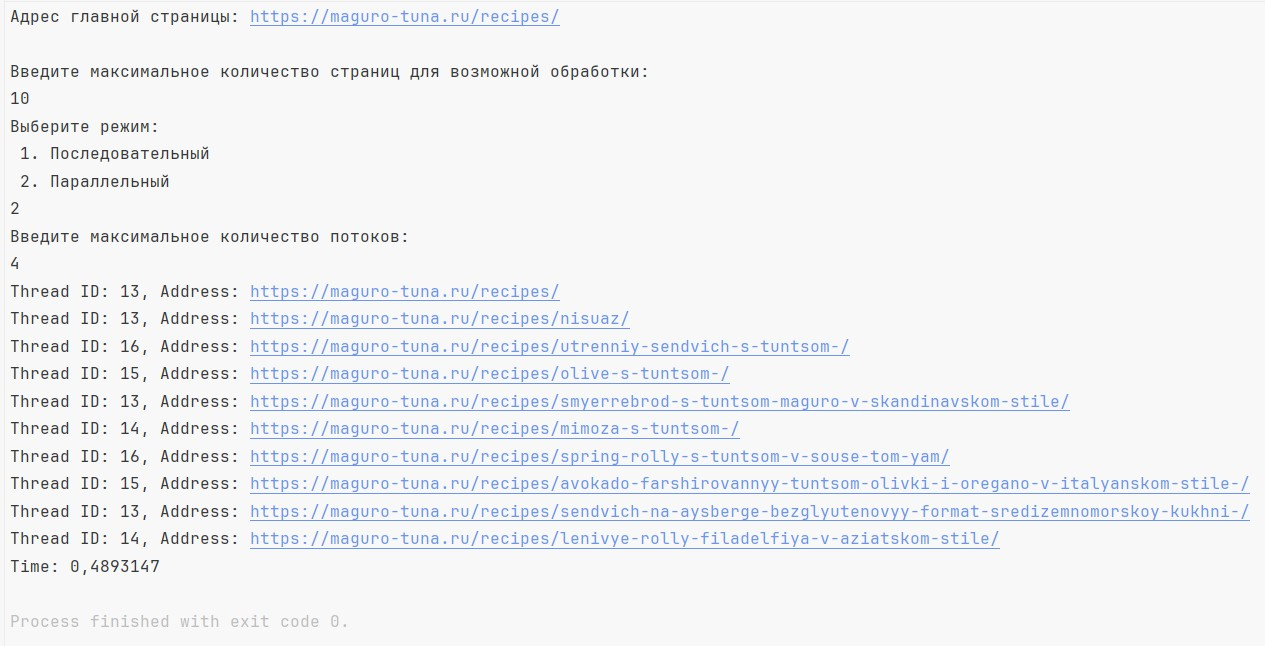
\includegraphics[width=170mm]{images/working_prog}
    \caption{Пример работы программы.}
    \label{images:working_prog}
\end{figure}


\vspace{20mm}
\chapter{Описание исследования}
Целью исследования является выявление оптимального числа потоков для максимальной производительности на многопроцессорной системе с четырьмя ядрами.

Замеры работы программы на разном количестве потоков и разном количестве страниц представлены в таблице~\ref{tbl:perf_tests}.

\begin{longtable}{|p{3.5cm}|p{3.5cm}|p{5cm}|p{3cm}|}
\caption{Среднее время выполнения и процентное ускорение работы программы} \label{tbl:perf_tests} \\ 
\hline
Кол-во потоков & Кол-во страниц & Среднее время выполнения (с) & Ускорение (\%) \\ 
\hline
\endfirsthead

\hline
Кол-во потоков & Кол-во страниц & Среднее время выполнения (с) & Ускорение (\%) \\ 
\hline
\endhead

\hline
\endfoot

\endlastfoot

1 поток & 1  & 0,10 & 100  \\ 
        & 11 & 0,66 & 100  \\ 
        & 21 & 1,27 & 100  \\ 
        & 31 & 2,20 & 100  \\ 
        & 41 & 2,84 & 100  \\ 
        & 51 & 3,06 & 100  \\ 
\hline
2 потока & 1  & 0,06 & 167  \\ 
         & 11 & 1,41 & 47   \\ 
         & 21 & 1,29 & 98   \\ 
         & 31 & 0,97 & 227  \\ 
         & 41 & 1,31 & 217  \\ 
         & 51 & 1,54 & 199  \\ 
\hline
4 потока & 1  & 0,05 & 200  \\ 
         & 11 & 1,16 & 57   \\ 
         & 21 & 1,23 & 103  \\ 
         & 31 & 1,14 & 193  \\ 
         & 41 & 1,24 & 229  \\ 
         & 51 & 1,09 & 281  \\ 
\hline
8 потоков & 1  & 0,05 & 200  \\ 
          & 11 & 1,18 & 56   \\ 
          & 21 & 1,17 & 109  \\ 
          & 31 & 1,17 & 188  \\ 
          & 41 & 1,19 & 239  \\ 
          & 51 & 1,46 & 210  \\ 
\hline
16 потоков & 1  & 0,06 & 167  \\ 
           & 11 & 1,35 & 49   \\ 
           & 21 & 1,26 & 101  \\ 
           & 31 & 1,25 & 176  \\ 
           & 41 & 1,40 & 203  \\ 
           & 51 & 1,24 & 247  \\ 
\hline

\end{longtable}

Результаты вычисления среднего ускорения работы программы при разном количестве потоков представлены в таблице~\ref{tbl:average_speedup}.

\begin{table}[h!]
\centering
\caption{Среднее ускорение работы программы в зависимости от количества потоков}
\label{tbl:average_speedup}
\begin{tabular}{|c|c|}
\hline
Кол-во потоков & Среднее ускорение (\%) \\ 
\hline
1 поток        & 100.00 \\ 
2 потока       & 159.17 \\ 
4 потока       & 177.17 \\ 
8 потоков      & 167.00 \\ 
16 потоков     & 157.17 \\ 
\hline
\end{tabular}
\end{table}


\section*{Общая формула}
Ускорение вычисляется по формуле:
\begin{equation}
\text{Ускорение (\%)} = \left( \frac{T_{\text{1 поток}}}{T_{\text{n потоков}}} \right) \times 100
\end{equation}

где:
\begin{itemize}
    \item \(T_{\text{1 поток}}\) — среднее время выполнения в последовательном режиме (1 поток),
    \item \(T_{\text{n потоков}}\) — среднее время выполнения в параллельном режиме (n потоков).
\end{itemize}

\section*{Пример расчёта}
Для 2 потоков и 1 страницы:
\begin{equation}
\text{Ускорение (\%)} = \frac{0.10}{0.06} \times 100 = 166.67\%.
\end{equation}


По результатам исследования построены графики времени выполнения программы и ускорения работы в зависимости от количества потоков~\ref{images:Graphics}.
\begin{figure}[H]
    \centering
    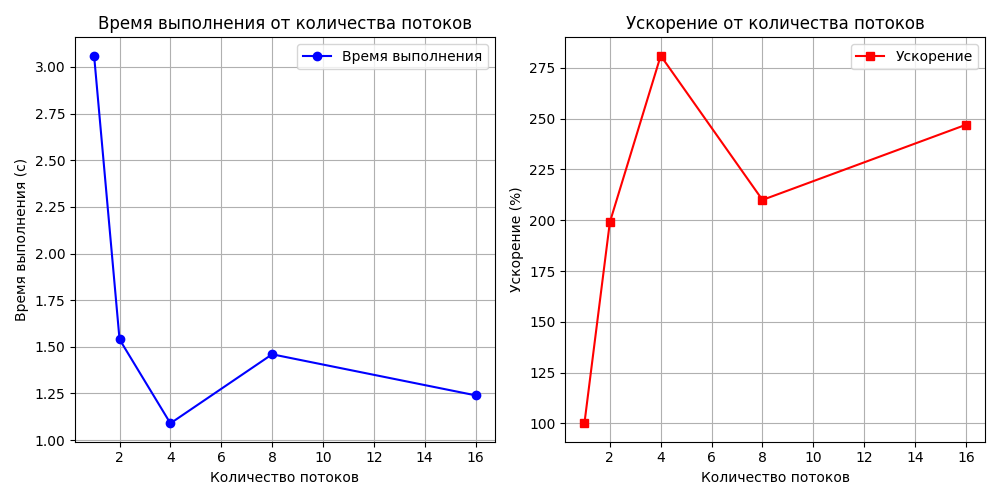
\includegraphics[width=170mm]{images/Graphics}
    \caption{Графики времени выполнения программы и ускорения работы в зависимости от количества потоков.}
    \label{images:Graphics}
\end{figure}

Технические характеристики устройства:
\begin{itemize}
    \item процессор: Intel(R) Core(TM) i5-10300H с тактовой частотой 2.5 Ггц;
	\item ядра: 4;
	\item логических процессоров: 8.
\end{itemize}


Вывод: при количестве потоков, равных количеству ядер процессора (4 ядра) производительность наибольшая.





\clearpage
\ssr{ЗАКЛЮЧЕНИЕ}

Цель работы достигнута. Разработано программное обеспечение, которое позволяет осуществлять параллельную выгрузку данных с интернет-ресурсов с использованием нативных потоков. Проведено исследование зависимости производительности программы от количества потоков и количества страниц. Полученные результаты показывают, что использование потоков значительно ускоряет выполнение задачи до предела в 4 потока (количество ядер).

Выполнены следующие задачи: 
\begin{itemize} 
	\item исследована предметная область; 
	\item разработан и реализован алгоритм параллельной обработки данных; 
	\item реализовано ПО на основе нативных потоков; 
	\item проведены тесты производительности. 
\end{itemize}